\chapter{Generation of a DSL Syntax}
\par
The Syntax of the DSL is the most important part of the project, as it is the place in the toolchain, where the modeller actually does his work: writing a model. Therefore the main requirement for the DSL is that the modeller, must be able to express all the functionalities needed for his models. On the other side, the syntax of the DSL must be as straightforward and intuitive as possible, so that the modeller can concentrate on his scientific activity and must only invest a small amount of time to learn and handle the DSL \autocite{dsl:mernik}.
\par
It is difficult to develop a DSL, with such a balance, in one step. Therefore the approach was to develop an easier DSL in the first place. Afterwards this DSL was used to develop simple existing models. Through that development the created DSL syntax could be validated. With this newly gathered modeling experience, it was possible to evaluate the syntax and the missing features of the DSL and to improve it in the next iteration of the same procedure.
The Similie tutorials were used as a starting point, for the first DSL draft. Similie and its tutorials were chosen over the other analysed frameworks because they had a clear structure and were well explained.
\par
With this approach, two DSL drafts were created. After the second draft, we realised that, it would not be possible to create our own DSL. Thus we tried to find another modelling DSL which already covers some needed features and provides us with a clear and structured syntax, which we finally could extend.
\par
In this section the two created drafts are described, then our chosen candidate DSL, Ocelet, is introduced and finally necessary extensions to Ocelet are specified.

\section{First DSL Draft}
\par
The first draft is a DSL that has the necessary functions to describe the bank-account model from the Similie \autocite{dsl:similie_tutorial_bank} tutorial. The attempt was to create a DSL with Xtext, a framework for DSLs, and to bind the DSL with an ontology.  
\par
For this first draft a practical approach was chosen, although this is not essential for a feasibility study. Nevertheless further insights and ideas were gained for the general DSL generation, by making the first steps for creating a DSL with Xtext. Thereby it could finally determined, that any implementation of runnable code from an own DSL, was completely out of scope for this project. This was due that, lots of DSL creation challenges appeared, which were partially hard to solve but mainly consisted of diligence work. These challenges were not relevant for the further proceeding, and therefore we stopped the concrete implementation at some point.\\
Another goal was to bind the DSL with an ontology, by that it would have been shown that if this works for a simple example, the same principle could also be applied for more complicated cases. 

\subsection{Implementation}
\par
To understand the further thoughts, it is necessary to comprehend the Similie Bank model shown in the diagram \ref{fig:simile_bank_account} below:
\begin{figure}[h]
	\centering
	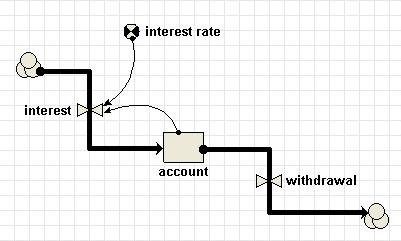
\includegraphics[width=0.7\textwidth]{pics/generation_of_a_dsl/similie_bank_account.png}
	\caption{Simile Bank Account \label{fig:simile_bank_account}}	
\end{figure}
\par
In detail, the diagram shows a compartment with the name $account$, the compartment has a value which represents the account balance. $Account$ has the starting value: $20$. It further shows a variable $interest\:rate$, which has a constant value. In this example it is $0.1$. There are also two flows in the picture. A flow adds or subtracts a certain value of a compartment, depending if it flows into to the compartment or out of it. The value is calculated by a formula the user entered. The two arrows are so called influences, they represent that the value of $account$ and $interest\:rate$ can be used in the formula of the $interest$ flow. The formula of $interest$ is $interest rate * account$ and that of withdrawal is $20$.
\par
Simile can convert this diagram into an executable program, which simulates this bank account. The principle of that program is, that every value will be recalculated for each timestep, based on the previous value. The user can enter how many timesteps will be calculated. In pseudo-code the main logic of the program could look like this:
\begin{verbatim}
interest_rate = 0.1
account = 20
timestep = 100
for each timestep:
	account = account + (interest rate * account)
	account = account - (20)
\end{verbatim}
\par
Of course this is not everything Simile does, as it is also responsible for I/O like drawing diagrams and so on. Nevertheless it should show, what is done at the first glance.\\
Our first DSL had the goal to be able to represent this diagram textually, so the bank account example described with the the DSL looks like the following:
\begin{verbatim}
Model bankAccount:
Container account INT = 200;
FlowIN INT interest TO account = interest_rate * account;
FlowOUT INT withdrawal FROM account = 20;
Conjunction interest_rate -- interest;
Conjunction  account -- interest;
variable INT interest_rate  = 0.1 ;
\end{verbatim}
\par
This way of describing a model has several flaws, which mostly result  from the fact that the DSL tries to mimic functionality that works for a visual modelling but not necessarily for a text based description of a model.
\par
The first problem is the use of conjunctions, which represent influences in Similie. In Similie they are needed to make values visible in the components where they should be used. For example: if the arrow from $account$ to $interest$ does not exist, the value from $account$ could not be used in the formula to calculate $interest$.\\
Therefore in our syntax the conjunctions are used to define the scope of use of variables and containers. This concept is widely known in programming as visibility rules. Defining every conjunction between variables, flows and containers with 1to1 relations is not practicable. If such visibility rules are needed a more effective way must be found.
These relationships serve another purpose in the execution of the model. By calculating the dependencies, the execution order in a model is determined. Without dependency definitions by the modeler, the calculation of dependencies and the execution of the model is bound to much more effort in the code generator.
\par
The next problem is the readability. A direct conversion of a visual modeling language to a textual does not produce a DSL with a readability that is necessary for a useful DSL. The conclusion is that a new concept for a DSL is necessary.
\par
The description of a model with a DSL is followed by the generation of executable code. XText already offers a mechanism to implement such a code generator, but the conceptual problems were too complex, so that no executable code generation was achieved. To overcome these conceptual complexity, deeper experience with code generation and compilers is needed. Nevertheless, with this experiment with XText we got a feeling, on what is possible with a DSL, and what is not. 
\par
An effort to find a way to integrate unit conversion with the help of ontologies into the code generation led to a small example, a Java standalone program, where the information on how to convert degree Kelvin to Celsius and vice versa is extracted from NASA Sweet ontologies. The example could not be tested with the DSL because of the problems with the code generator, but experience with information extraction from ontologies was gained. In principle it is possible to make such connections to the ontologies and to bind the data types with semantic. 
\par
The result of this example is that the code generation is out of scope for this project and that a new DSL definition is necessary, because a textual DSL has other requirements than a visual modeling like Simile. Though we went on to the second DSL draft.

\subsection{Second DSL Draft}
\par
In our second DSL draft we decided to follow the explanations in the Paper ``Declarative Modelling'' from \autocite{dsl:muetzelfeldt}. So we have chosen to define our DSL in a declarative way. That means that, in the most cases, there is no need to write instructions how to calculate some values. The goal is to describe all calculations with describe statements as a mathematical formula. These describe-statements of the calculations can be separated from the concrete model. That means the concrete model uses the formulas which was described earlier or are available in a database/ontologie.
\par
Each describe-statement defines a mapping between a new value set and a value set that is used to generate it. This idea includes some advantages known from functional programming languages:
\begin{enumerate}
	\item Facilitated model verification: In fact that Describe Statements does not accesses the memory, since they are defined declaratively.
	\item Usability: The modeller, often with a strong mathematical background, is able to write his models in a way that is familiar to him by using formulas instead of instructions. The fact that the code is easier to write accompanies the advantages that the code is also easier to read.
\end{enumerate}
Once we have described all necessary mathematical functions/mappings in our DSL we have to bring these mappings together in an executable model. To run a model  we need to describe each iteration. At this point we break with the declarative paradigm and use an imperative style to define each iterations.
%TODO Referenz suchen.
An imperative approach brings the advantage that we have an random access to values calculated in previous iterations and we are able to pass the results of the current iteration to the next iteration. \\
The bank account model implemented in the DSL would look something like this:
%TODO Syntax hervorheben
\begin{verbatim}
describe interest_rate depends on timestep as 1 end
describe q depends on interest_rate as 1+interest_rate/100 end
describe withdrawal depends on timestep as 50 end
describe balance depends on q, withdrawal, old_balance as
old_balance * q - withdrawal
end
run simulation from 1..10
    init tmp_balance = 1000 do
	tmp_balance = balance(q(interest_rate), withdrawal, tmp_balance)
end
\end{verbatim}
\par
In the code above it is recognizable that the $describe$ statement is used to define a mathematical function. In the example $interest\_rate$ depends on timestep. Described in mathematical terms:\\
$interest\_rate(timestep) : \mathbb{N} \rightarrow  \mathbb{R}$
\par
At the moment $interest\_rate$ maps every timestep to the value 1 but in reality the $interest\_rate$ changes in time. There is a possibility to describe the changes with a formula but in many cases there is no structure in the changes. For the case of $interest\_rate$ it should not be only possible to write mathematical expressions after the $describe$ statement, further it should possible to read the desired values from an array, a submodel or a database. So the $describe$ statement provides a way to plug datasources or other models into our models.
\par
Up to that point, we ignored the connection between the ontology and the syntax of the DSL. Nevertheless we wanted to try to build a sample model with that DSL, to get a feeling for it and perhaps get an idea how we could realise the connection to the ontology. So in the next step we tried to write a predator-prey model with the DSL.
\par
The predator-prey model was build after that one used in \autocite{dsl:dynamo}. The model with our syntax can be found in the [appendix].
%TODO ist das im Anhang etc. 
The resulting code is not finished but already bloated and therefore not readable and unintuitive.
\par
Because of those two points, missing connection to an ontologie and intuitiveness, we decided to research an already existing DSL for environmental modelling, which we could use as template.

\subsection{Ocelet}
\par
The result of that search was Ocelet. Ocelet is a modeling language and a development environment for landscape models. It was developed in the scope of the STAMP project, which stands for Modelling dynamic landscapes with Spatial, Temporal And Multi-scale Primitives. \autocite{dsl:ocelet-wiki} The project is supported by the ANR, the Agence Nationale de la Recherche. It started in 2007 and had a duration of 42 months, after which it was abandoned and is not in further development. We could not find out, if a follow-up project exists.
\par
The following information about Ocelet were found in \autocite{dsl:ocelet-design}. The goal of Ocelet is to allow the domain experts to concentrate on the conceptual model. The task of the transformation of the model to an executable implementation is left to an dedicated software tool.  \\
Though the design of Ocelet has the following two main points.
\begin{enumerate}
	\item It provides concepts adapted for the modelling processes, especially in the landscape sector.
	\item It must have underlying operational semantics that are required to automatically generate code and run simulations, which correspond to the models written in the Ocelet programming language. This means that Java code is generated from Ocelet code, thus a code generator are needed.
\end{enumerate}
To make the modeler’s work easier, Ocelet provides a model building environment, which enables syntax analysing and type verification, which is standard in most other common programming languages. \\
Furthermore the model needs to be executed, so Ocelet also provides a program execution platform based on component-service technologies. \\
A schematic overview of Ocelet can be seen in the diagram \ref{fig:ocelet_modelling_and_simulation_framework} below, it is taken from \autocite{dsl:ocelet-design}.
\begin{figure}[h]
	\centering
	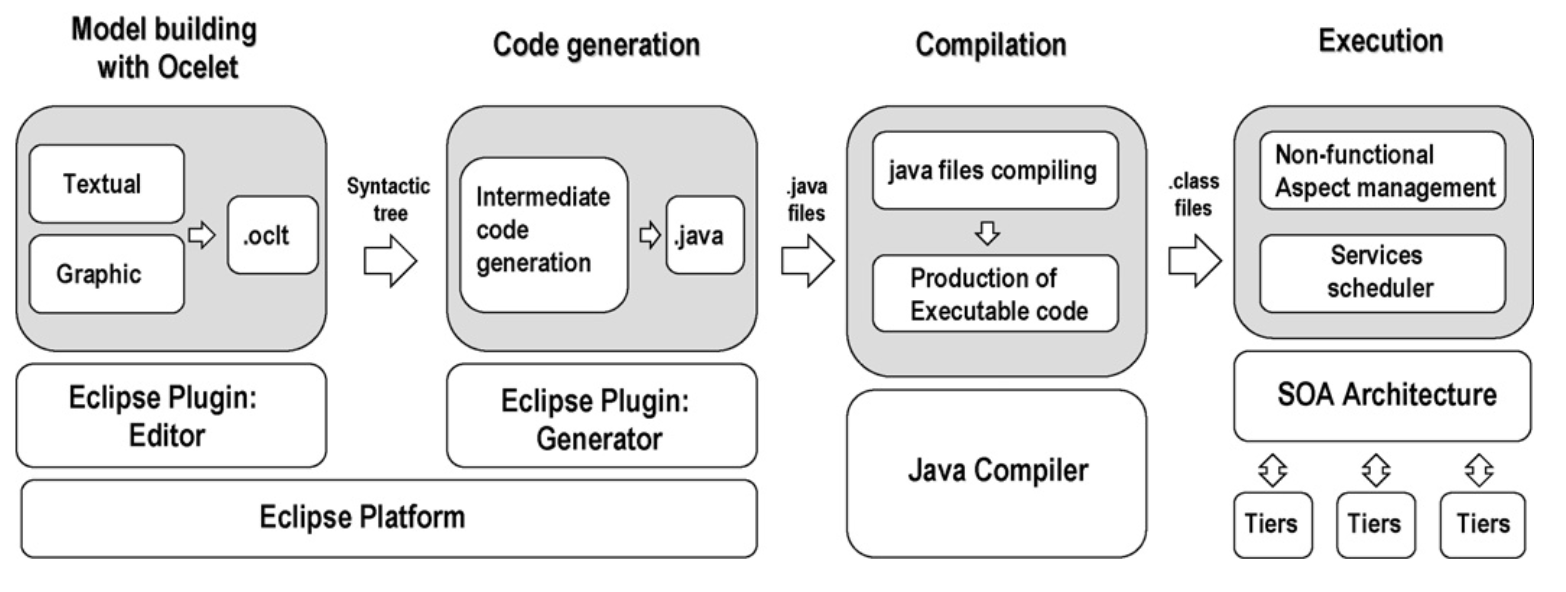
\includegraphics[width=1.0\textwidth]{pics/ocelet/ocelet_modelling_and_simulation_framework.png}
	\caption{A schematic overview of Ocelet \label{fig:ocelet_modelling_and_simulation_framework}}	
\end{figure}

\subsubsection{Modelling paradigm}
\par
As already described Ocelet is an own DSL, where the code is translated to Java, which then can be executed on the computer.\\
Ocelet was build around of 5 main concepts:
\begin{itemize}
	\item entity
	\item service
	\item relation
	\item scenario
	\item datafacer
\end{itemize}
These concepts are further explained in more detail subsequently. Of course Ocelet also knows other common concepts like arguments, properties and numbers, which will not be explained in detail in this document.
\par
The following definitions of the 5 main concepts are taken from \autocite{dsl:ocelet-onto} and \autocite{dsl:ocelet-design} respectively.
\emph{
\paragraph{Entity}
Entities are basic modelling parts that can be put together to build a model. A whole model is, as such, also an entity. An entity can contain other entities, and is then called a composite entity. Entities that do not contain other entities are called atomic entities. An entity is able to store information using attributes. An entity communicates with its environment through input and output ports named services.\\
For example: A forest can be modelled by a composite entity that contains tree entities which are part of the forest. And each tree can have an age attribute.
\paragraph{Service}
A service is a communication port of an entity. It is an input service when it accepts input values or events from other entities and it is an output service when it exports values or events to other entities.\\
Services are defined like functions: they have a name, accept arguments, can produce results.
\paragraph{Relation}
A relation is the expression of how a set of entities relate to each other at a given moment. Hence a relation definition describes which entities can be related and also contains a functional part which describes what is happening when they interact.
\paragraph{Scenario}
A scenario gives a description of which actions and relations within a composite entity have to be activated, and when. The relations in turn put selected entities in interaction in space and time. The scenario therefore expresses the spatial and temporal internal behaviour of a composite entity by managing the entities and relations it contains. For example, a ten-year evolution scenario embedded in a village entity could describe the extension of the village by a few houses every year, taking in account population growth and several policy rules that govern spatial expansion. The ten-year scenario could also be composed of yearly evolution scenarios.
\paragraph{Datafacer}
A datafacer is a component through which entities access data. The aim of datafacers is to abstract access methods to the entities. In the domain of geographical information, a datafacer can take the form of an external database, a satellite image repository or an internal logfile.
}
\par
In \autocite{dsl:ocelet-design} the creators of Ocelet show that these five concepts are enough to represent most of the situations, which occur in dynamic landscape modeling. Although it is not proven if these concepts are also sufficient to represent most environmental models, which are not directly connected to the landscape.

\subsubsection{Ocelet and Ontologies}
\par
According to \autocite{dsl:ocelet-design} an ontology can be mapped to Ocelet code and vice versa. This is shown in diagram \ref{fig:ocelet_and_ontologies}.
\begin{figure}[h]
	\centering
	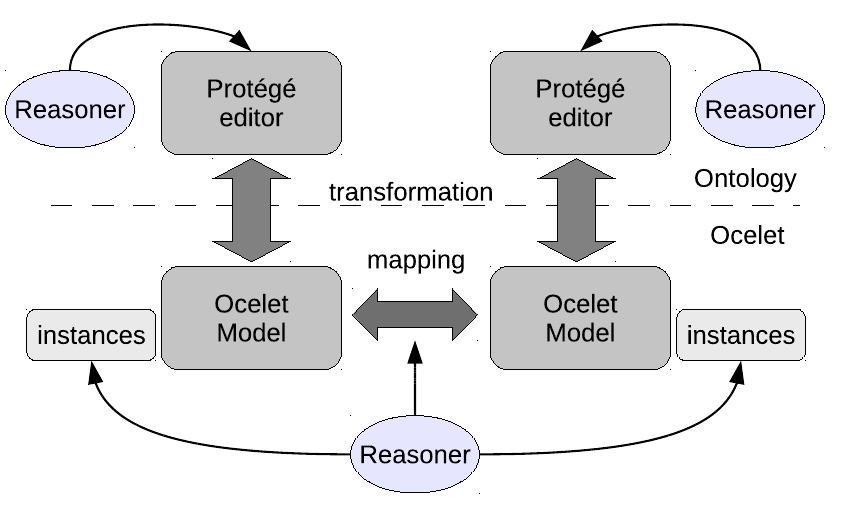
\includegraphics[width=0.7\textwidth]{pics/ocelet/ocelet_and_ontologies.png}
	\caption{Ocelet models and Ontologies  \label{fig:ocelet_and_ontologies}}	
\end{figure}
\par
In the image it is shown that a model can be mapped to an equivalent model in an ontology. Furthermore the mapping is fully automated and therefore does not require any actions of the end-user. This has the advantage that the model can be checked for inconsistencies with a reasoner. Although the modeler can be warned about such inconsistencies, it is not possible, to automate the repair process, as it is a nondeterministic process.  
\par
Another advantage is that parts of one model can be easily reused in other models, as for example an entity in one model can be an equivalent, specialisation or generalization of an entity in an other model.

\subsubsection{Missing features of Ocelet}
\par
For our use, Ocelet has two main shortcomings. In the first place, Ocelet does not follow an universal approach as it only focuses on landscape modelling. Secondly, Ocelet models can be reasoned with ontologies, but this feature is not as extensive as we need it.

\par
In the next section, we describe therefore how Ocelet could be enhanced for our needs.














